\section{Background}
\label{background}

\subsection{Forensics eco-system}
One of the challenges encountered every day on forensic research is the large and heterogeneous collection
of libraries, tools, and data available to us. Our project designs and prototypes solutions for the
integration of many existing components into a single system which is flexible, robust and effective for
forensic data exploration.

External libraries have may years of domain knowledge which is not easily converted into a
realtional query. They are part of a long and complex pipe-line which can't all be replaced
by a relational or a series of relational queries. The access to external repositories to
consume data and feed results back to visualization tools or data services turns the
conversion of the pipeline into series of relational queries even more complex.

\subsection{Hadoop eco-system}

\begin{figure}[lb]
%\vspace*{-5mm}
\centering
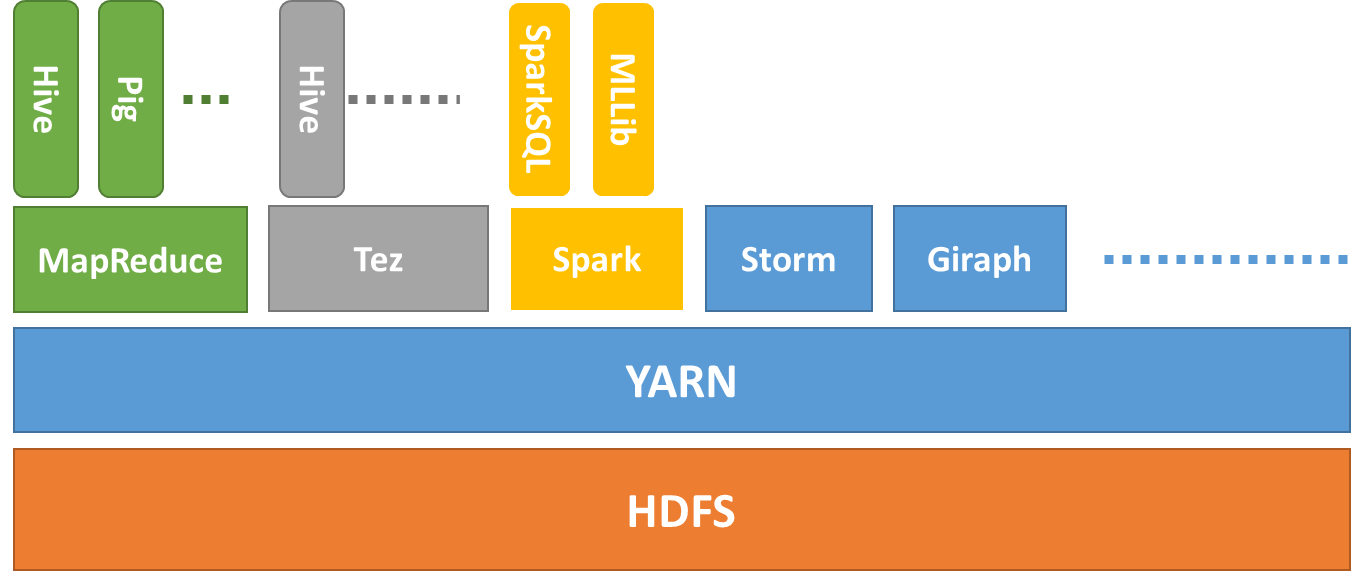
\includegraphics[width=.48\textwidth]{fig/hadoop_2.png}
\caption{Hadoop 2.0}
\label{haddop_2}
\end{figure}


\subsection{Docker Containers}
Docker combines an easy-to-use interface to Linux containers with easy-to-construct image files for those containers. In short, Docker launches very light weight virtual machines.

According to the Docker website, “Docker is an open platform for developers and sysadmins to build, ship, and run distributed applications. Consisting of Docker Engine, a portable, lightweight runtime and packaging tool, and Docker Hub, a cloud service for sharing applications and automating workflows, Docker enables apps to be quickly assembled from components and eliminates the friction between development, QA, and production environments.”, www.docker.com. For more information how how virtualization works and how docker differs from virtual machines check link and its user guide. More info is available at the Docker workshop gitHub.


